\documentclass[elementsmain.tex]{subfiles}
\begin{document}
\section{Lines, Especially in $\mathbb{R}^2$}

We will need a good understanding of lines in $\R^n$. We shall introduce lines
with a geometric definition using vectors, and then show how to describe a line as the 
image of a parametric curve. Finally, we will focus on just the plane $\R^2$, and see
how to describe a line as the set of solutions to an equation.

\subsection*{Lines as Parametrized Objects}

Any pair of points should define a line. In $\R^n$, we can do this using vectors.
It will be fruitful to regularly conflate a point with the (mathematician's) vector having the point as its head, so we will do that throughout this section.

\begin{definition}[Lines in $\R^n$]
Suppose that $P$ and $Q$ are two distinct vectors in $\R^n$. We say that a point $X$ \emph{lies on the line through $P$ and $Q$} when there exists scalars $\lambda$ and $\mu$ which are not both zero so that
\[
\lambda (X-P) = \mu (X-Q).
\]
The \emph{line through $P$ and $Q$} is the set of all such points, that is, it is the set
\[
\begin{split}
&\left\{ X  \in \R^n \,\middle|\, \text{$X$ lies on the line through $P$ and $Q$}\right\} \\
& = \left\{ X\in\R^n \,\middle|\, \lambda(X-P) = \mu(X-Q), \text{for some $\lambda$ and $\mu$ where $\lambda\mu\neq0$} \right\}
\end{split}
\]
\end{definition}

Of course, we want $P$ and $Q$ to both lie on the line through $P$ and $Q$. Fortunately, this is true.

\begin{theorem}
Let $P$ and $Q$ be distinct vectors in $\R^n$. Then both $P$ and $Q$ lie on the line through $P$ and $Q$.
\end{theorem}

\begin{proof}
We will show that $P$ lies on the line through $P$ and $Q$. 
We must check the condition from the definition with $X$ replaced by $P$. This means we want to know about the vectors $X-P$ and $X-Q$, when $X=P$. But $P-P=0$, so we can just choose $\lambda = 1$ and $\mu=0$, and get the equation 
\[
\lambda (X-P) = 1 (P - P) = 0 (P - Q) = \mu (X-Q) .
\]

The proof that $Q$ lies on the line through $P$ and $Q$ is basically the same, with some of the letters moved around. I will leave it to you to check the details of that case.
\end{proof}


\begin{theorem}[Only One Direction Matters] \label{thm:one-direction}
Let $P$ and $Q$ be two distinct vectors in $\R^n$.
A vector $X\in\R^n$ lies on the line through $P$ and $Q$ if, and only if, there exists a scalar $t$ so that $X-P = t(Q-P)$.
\end{theorem}

\begin{proof}
First suppose that $X$ lies on the line through $P$ and $Q$. Then, by definition there exists a pair of scalars $\lambda$ and $\mu$ so that 
\begin{equation}\label{eq:1-5-one-direction}
\lambda(X-P) = \mu(X-Q).
\end{equation}
Notice that we cannot have $\lambda=\mu$. The reason is that if $\lambda = \mu \neq 0$, then we can cancel them and deduce that $X-P = X-Q$, which means that $P=Q$. But we have explicitly chosen $P$ and $Q$ to be distinct. So, we will proceed knowing that $\lambda$ and $\mu$ are different.

Rearranging equation (\ref{eq:1-5-one-direction}) , we see that
\[
(\lambda-\mu)X - \lambda P = -\mu Q.
\]
By adding $\mu P$ to both sides and gently regrouping things, we find
\begin{align*}
(\lambda - \mu) X -\lambda P + \mu P &= - \mu Q + \mu P \\
(\lambda - \mu) X - (\lambda -\mu)P &= -\mu (Q - P) \\
(\lambda - \mu) (X - P) &= -\mu (Q - P)
\end{align*}
Since $\lambda - \mu \neq 0$, we can divide by it, and we see that
\[
X - P = \dfrac{-\mu}{\lambda-\mu} (Q-P).
\]
So we can choose $t = \dfrac{-\mu}{\lambda-\mu}$ to satisfy the condition of the theorem.

Now suppose that $X$ is a point so that $X-P = t (Q-P)$ for some scalar $t$.
We must find the scalars $\lambda$ and $\mu$ which satisfy equation (\ref{eq:1-5-one-direction}). Since $X-P = t(Q-P)$, we have that 
\begin{equation}\label{eq:symmetric-line}
X = tQ + (1-t)P
\end{equation}
This means that $X-Q = (t-1)(Q-P)$. So if we choose $\lambda = t-1$ and $\mu = t$, we have
\[
\begin{split}
\lambda (X-P) & = (t-1) (X-P) \\
		& = (t-1) t (Q-P) \\
		& = t (X-Q) \\
		& = \mu (X-Q).
\end{split}
\]
Therefore, $X$ lies on the line through $P$ and $Q$.
\end{proof}

Equation (\ref{eq:symmetric-line}) is a beautifully symmetric description 
for points $X$ which lie on the line through $P$ and $Q$. Many authors, especially 
those who want to do lots of geometry, emphasize this description.

Also, notice the importance this theorem places on the vector $Q-P$. This vector is
useful enough for dealing with the line that it has a special name.

\begin{definition}[Direction Vector]
Let $P$ and $Q$ be two distinct vectors in $\R^n$. The vector $Q-P$ is called a \emph{direction vector} for the line through $P$ and $Q$.
\end{definition}

The order of the points $P$ and $Q$ really doesn't matter for defining a line, so we can see that $P-Q$ is a direction vector, too. It just points in the opposite direction. Furthermore, a line has lots of points on it, and any pair of them is good enough to 
describe the line. Choosing a different pair for $P$ and $Q$ will lead to different direction vectors, but only different by rescaling. All of the vectors will point in the same direction. So keep in mind that a line has lots of direction vectors, but only one direction.

\begin{corollary}[Parametric form of a Line]\label{cor:parametric-line}
Let $P$ and $Q$ be two distinct vectors in $\R^n$. The line through $P$ and $Q$ is the set
\[
\left\{ X \in \R^n \,\middle|\, X = P + t(Q-P) \text{ for some scalar $t$}\right\}.
\]
\end{corollary}

\begin{proof}
This condition is a simple rearrangement of the one in Theorem \ref{thm:one-direction}. Just add $P$ to both sides of the description there.
\end{proof}

\begin{corollary}[Lines through the origin]
A line in $\R^n$ can be written in the form
\[
\left\{ X \in \R^n \,\middle|\, X = t V \right\},
\]
where $V$ is some fixed vector.
\end{corollary}

\begin{proof}
Essentially, this is the case where $P=0$. We replace $Q = Q-P$ by $V$.
\end{proof}

Note that the vector $X = P + t(Q-P)$ changes as $t$ changes. We often think of this as
defining a function of the form $\gamma: t \mapsto P + t(Q-P)$. (By the way, $\gamma$ is a version of a Greek letter and is read ``gamma.'') Usually, the best way is
to think of the number $t$, called the \emph{parameter}, as representing time. As the time $t$ changes, the vector $X = \gamma(t)$ moves around in $\R^n$. In the case here, 
the point $X=\gamma(t)$ traces out the shape of a line as time moves on. 

If you prefer to think about the whole vector $\gamma(t)$, rather than just its head, it helps to imagine that vector sweeping through space as time goes on. The heads of the vectors still trace out the line, but the tails of the vectors all stay at the origin.

\begin{figure}[h!]
\centering
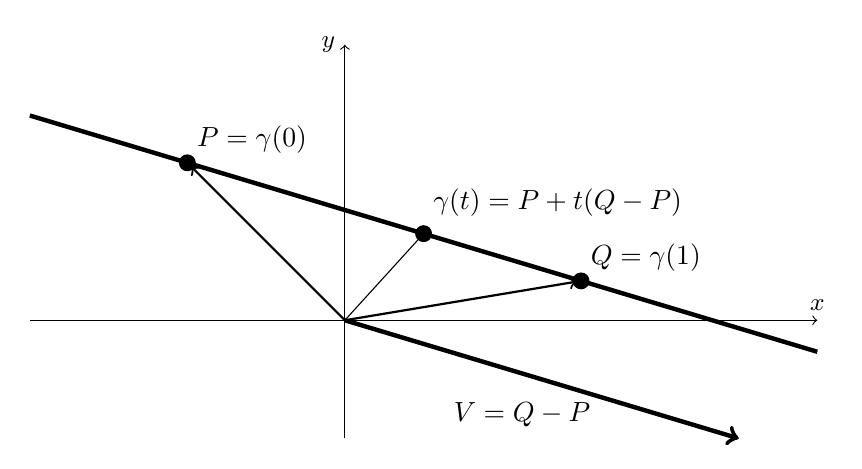
\begin{tikzpicture}[scale=1]
\draw[->] (-4,0) -- (6,0) node[above] {\small $x$};
\draw[->] (0,-1.5) -- (0,3.5) node[left] {\small $y$};
\draw[fill] (-2,2) circle [radius=.1];
\node[above right] at (-2,2) {$P = \gamma(0)$};
\draw[fill] (3,.5) circle [radius=.1];
\node[above right] at (3,.5) {$Q =\gamma(1)$};
\draw[ultra thick] (-4,2.6) -- (6,-.4);
\draw[fill] (1,1.1) circle [radius=.1];
\draw[->] (0,0) -- (1,1.1);
\node[above right] at (1,1.2) {$\gamma(t) = P + t(Q-P)$};
\draw[->,thick] (0,0) -- (-1.95,1.95);
\draw[->,thick] (0,0) -- (2.94,.49);
\draw[->,ultra thick] (0,0) -- (5,-1.5);
\draw (0,0) -- (5,-1.5) node[midway,xshift=-.25cm,yshift=-.45cm] {$V = Q-P$};
\end{tikzpicture}
\caption{parametric line and a direction vector}
\label{fig:param-line2}
\end{figure}

You might see parametric functions in other places (like a course on calculus),
but written differently. It is common to break apart a vector description into a system of component functions. We will have occasion to use this, too, so let's see how it is done. Begin with a parametric line 
\[
\gamma(t) = P + t (Q-P).
\] 
Write out the vectors $\gamma(t)$, $P$ and $Q$ as stacks of components, 
\[
\gamma(t) = \begin{pmatrix} x_1(t) \\ x_2(t) \\ \vdots \\ x_n(t) \end{pmatrix}
\qquad
P = \begin{pmatrix} P_1 \\ P_2 \\ \vdots \\ P_n \end{pmatrix}
\qquad
Q = \begin{pmatrix} Q_1 \\ Q_2 \\ \vdots \\ Q_n \end{pmatrix}
\]
and unpack the definition using the algebra of linear combinations.
\[
\begin{pmatrix} x_1(t) \\ x_2(t) \\ \vdots \\ x_n(t) \end{pmatrix}
= \begin{pmatrix} P_1 \\ P_2 \\ \vdots \\ P_m \end{pmatrix} 
+ t \begin{pmatrix} Q_1-P_1 \\ Q_2-P_2 \\ \vdots \\ Q_n-P_n \end{pmatrix}
= \begin{pmatrix} P_1 + t (Q_1-P_1) \\ P_2 + t (Q_2-P_2) \\ \vdots \\ P_n + t (Q_n-P_n) \end{pmatrix}
\]
Now, just read off each component, one at a time, to make a system of functions. It sounds like cheating, but you basically just erase the parentheses and then group with a big curly brace on the left instead.
\begin{equation*}
\left\{\begin{array}{ccc}
x_1 & = & P_1 + t(Q_1 - P_1) \\
x_2 & = & P_2 + t(Q_2 - P_2) \\
\vdots & & \vdots \\
x_n & = & P_n + t(Q_n - P_n)
\end{array}\right.
\end{equation*}

Sometimes people will write $x_i(t)$ with the parameter $t$ explicitly present, and sometimes they will write just $x_i$ and leave it as understood that $x_i$ is a function of $t$. I have left the $t$'s out of the final expression because it was convenient.


\subsection*{Implicit Description: The Equation of a Line in $\R^2$}

Now we narrow our attention to the plane $\R^2$. We will see that in this case
it is possible to also describe a line as the set of points satisfying a single, 
simple equation.

\begin{theorem}
Let $P$ and $Q$ be two distinct vectors in $\R^2$. Then there are numbers $a$, $b$, and $c$ so that any point $X = \left(\begin{smallmatrix} x \\ y \end{smallmatrix}\right) \in \R^2$ which lies on the line through $P$ and $Q$ must satisfy the equation
\[
ax + by = c.
\]
\end{theorem}

\begin{proof}
Let $P$ and $Q$ have components as follows:
\[
P = \begin{pmatrix} P_1 \\ P_2 \end{pmatrix}
\qquad
Q = \begin{pmatrix} Q_1 \\ Q_2 \end{pmatrix}
\]
By the discussion at the end of the last subsection, we can find a value of $t$ so that 
\[
\left\{ \begin{array}{ccc}
x & = & P_1 + t(Q_1 - P_1) \\
y & = & P_2 + t(Q_2 - P_2) .
\end{array}\right.
\]
Our goal is to eliminate $t$ from these expressions and derive a single equation relating $x$ and $y$. The mechanics of this is as follows: multiply the first equation through by $Q_2-P_2$, multiply the second equation through by $-(Q_1-P_1)$, and then add them. In a way, we are making a ``linear combination of the equations.'' The result is
\begin{equation}
\label{eq:1-5-eliminated}
\begin{split}
(Q_2-P_2) x - (Q_1-P_1) y & = (Q_2 - P_2) P_1 - (Q_1-P_1) P_2 \\
&  = Q_2 P_1 - Q_1P_2
\end{split}
\end{equation}

So, we choose $a = Q_2-P_2$, $b= -(Q_1-P_1)$ and $c = Q_2 P_1 - Q_1P_2$. Then equation (\ref{eq:1-5-eliminated}) reads as $ax + by = c$. This completes the proof.
\end{proof}


\begin{theorem}\label{thm:param-to-eqn}
Fix numbers $a$, $b$, and $c$ so that $a$ and $b$ are not both zero. Then the set of points $X = \left(\begin{smallmatrix} x \\ y \end{smallmatrix}\right)$ which satisfy the equation $ax+by=c$ is a line in $\R^2$.
\end{theorem}

\begin{proof}
We will work in the case where $a\neq 0$, and leave the case $a=0$ for you to fill in.

The main idea is to turn the defining equation into a parametric description, and along the way find vectors to play the parts of $P$ and $V = Q-P$. 

We will pretend that $y$ is our parameter by giving it a new name. So, introduce the parameter $t$ and declare that $y=t$. Take the defining equation $ax+by=c$, isolate $x$ and substitute in $y=t$ to remove reference to $y$. Then our information is represented by these two equations.
\[
\left\{\begin{array}{rrrrr}
x & = & c/a & - & (b/a)\, t\\
y & = &  &  & t
\end{array}\right.
\]
Rewrite this as a vector equation.
\[
X = \begin{pmatrix} c/a \\ 0 \end{pmatrix} + t \begin{pmatrix} -b/a \\ 1\end{pmatrix}
\]
So if we choose $P$ and $Q$ as below, we have written exactly the parametric description of a line as in Corollary \ref{cor:parametric-line}. 
\[
P = \begin{pmatrix} c/a \\ 0 \end{pmatrix} \qquad Q = \begin{pmatrix} c/a - b/a \\ 1 \end{pmatrix}
\]
Therefore, our collection of points is exactly a line. This completes the proof. (You should go back and fill in how to think about the case when $a=0$. Hint: if $a=0$, what do you know about $b$?)
\end{proof}

Looking carefully at the last two results together, we see that lines in $\R^2$ come with two different descriptions, a parametric description and an implicit description, but we can easily pass back and forth between them. In fact, the proofs of the last two results give us explicit methods for passing back and forth between them. In the first, we eliminate the parameter. In the second, we have to introduce a new one out of nowhere.



\begin{theorem} \label{thm:dir-vec}
Let a line in the plane be described as the set of solutions to the equation $ax+by=c$. A direction vector for this line is 
\[
V = \begin{pmatrix} -b/a \\ 1 \end{pmatrix}.
\]
\end{theorem}

\begin{proof}
This follows directly from our work in the proof of Theorem \ref{thm:param-to-eqn}. 
\end{proof}

While direction vectors are useful for lines in $\R^2$, in $\R^n$ we will have other, bigger objects defined by equations. In those cases, a single direction vector will not be sufficient. But we can keep things simple by changing perspective just a little. 

\begin{definition}[Normal Vector] Suppose we have a line in $\R^2$ through points $P$ and $Q$. A vector $n$ is called a \emph{normal vector} for this line if $n$ is orthogonal to the direction vector $V= Q-P$. That is, $n$ is a normal vector when $n\cdot (Q-P) = 0$.
\end{definition}

\begin{theorem}
Let $\ell$ be a line in $\R^2$ defined as the set of solutions to the equation $ax+by =c$. Then one normal vector for $\ell$ is given by
\[
n = \begin{pmatrix} a \\ b \end{pmatrix}.
\]
\end{theorem}

\begin{proof}
By Theorem \ref{thm:dir-vec}, the direction vector for $\ell$ is $V = (\begin{smallmatrix} -b/a \\ 1 \end{smallmatrix})$. It is straightforward to check that
\[
n \cdot V = \begin{pmatrix}a \\ b \end{pmatrix} \cdot \begin{pmatrix} -b/a \\ 1 \end{pmatrix} = -b + b = 0.
\]
Therefore, $n$ is a normal vector for $\ell$.
\end{proof}

Note that the normal vector is pretty handy for writing out the equation of a line. If we write 
\[
n = \begin{pmatrix} a \\ b \end{pmatrix} \qquad X = \begin{pmatrix} x \\ y \end{pmatrix}
\]
then the equation $ax+by=c$ is the same thing as $n\cdot X = c$. This gives us a connection between the dot product and the linear equation which will be useful later.

\clearpage

\subsection*{Exercises}

\begin{exercise}
Write down five different points which lie on the line described parametrically as:
\[
t \mapsto \begin{pmatrix} -5\\3 \end{pmatrix} + t \begin{pmatrix}1\\-1/2\end{pmatrix}.
\]
Plot these points and the line.
\end{exercise}

\begin{exercise}\label{task:line-through-origin}
Write down a parametric description for the line which passes through the origin $O=(0,0)$ and the 
point $S = (-5,5)$.

Is this the \emph{only} way to write down such a parametric description for that line?
\end{exercise}

\begin{exercise}\label{task:line-through-points}
Write down a parametric description for the line which passes through the points below.
\[
 T = (\pi, 0), \qquad J = (0,-\pi)
\]
Now find a different parametric description for that line. (\emph{Hint: Can you find a way to write a parametric description that doesn't use the number $\pi$?})
\end{exercise}

\begin{exercise}
For each of the conditions below, either find an example of a $2$-vector $Z$ so that the equation
\[
\begin{pmatrix}1\\2\end{pmatrix} + t\begin{pmatrix}-1\\1 \end{pmatrix} = Z
\]
has the given number of solutions, or explain why such an example is not possible.
\begin{compactitem}
\item[a)] exactly zero solutions;
\item[b)] exactly one solution; 
\item[c)] exactly two solutions.
\end{compactitem}
\end{exercise}

\begin{exercise}
For each of the conditions below, either find an example of a $2$-vector $Y$ so that the equation
\[
\begin{pmatrix}-2/5\\2\end{pmatrix} + tY = \begin{pmatrix}-1\\1 \end{pmatrix} 
\]
has the given number of solutions, or explain why such an example is not possible.
\begin{compactitem}
\item[a)] exactly zero solutions;
\item[b)] exactly one solution; 
\item[c)] exactly two solutions.
\end{compactitem}
\end{exercise}

\begin{exercise}
What shape is the set of solutions $\left(\begin{smallmatrix} x \\ y \end{smallmatrix}\right)$ to the equation
\[
\begin{pmatrix} 3 \\ 7\end{pmatrix} \cdot \begin{pmatrix} x \\ y \end{pmatrix} = 5?
\] 
That is, if we look at all possible vectors $\left(\begin{smallmatrix} x \\ y \end{smallmatrix}\right)$
which make the equation true, what shape does this make in the plane? Draw this shape.

What happens if we change the vector $\left(\begin{smallmatrix} 3 \\ 7 \end{smallmatrix}\right)$ to some other vector? What happens if we change the number $5$ to some other number?
\end{exercise}

\begin{exercise}\label{task:norm-to-param}
We begin with a line described parametrically by
\[
t \mapsto \begin{pmatrix} 6\\ -\pi \end{pmatrix} + t \begin{pmatrix} 34 \\ -19/3\end{pmatrix}.
\]
\begin{compactitem}
\item[a)] Find a normal vector for this line.
\item[b)] Plot the line and the normal vector you found.
\item[c)] Find an equation for this line.
\end{compactitem}
\end{exercise}


\begin{exercise}\label{task:norm-to-eqn}
We begin with a line described by the equation
\[
-3x + y =7.
\]
\begin{compactitem}
\item[a)] Find a normal vector to the line
\item[b)] Plot this line and the normal vector you found.
\item[c)] Find a parametric description for this line.
\end{compactitem}
\end{exercise}






\clearpage


\end{document}